%%%%%%%%%%%%%%%%%%%%%%%%%%%%%%%%%%%%%%%%%
% Twenty Seconds Resume/CV
% LaTeX Template
% Version 1.1 (8/1/17)
%
% This template has been downloaded from:
% http://www.LaTeXTemplates.com
%
% Original author:
% Carmine Spagnuolo (cspagnuolo@unisa.it) with major modifications by
% Vel (vel@LaTeXTemplates.com)
%
% License:
% The MIT License (see included LICENSE file)
%
%%%%%%%%%%%%%%%%%%%%%%%%%%%%%%%%%%%%%%%%%

%----------------------------------------------------------------------------------------
%	PACKAGES AND OTHER DOCUMENT CONFIGURATIONS
%----------------------------------------------------------------------------------------

\documentclass[letterpaper]{twentysecondcv-eng} % a4paper for A4
\usepackage[english]{babel}
\selectlanguage{english}
\usepackage[utf8]{inputenc}
%----------------------------------------------------------------------------------------
%	 PERSONAL INFORMATION
%----------------------------------------------------------------------------------------

% If you don't need one or more of the below, just remove the content leaving the command, e.g. \cvnumberphone{}

\profilepic{../img-shared/profile1.jpeg} % Profile picture

\cvname{Luis} % Your name
\cvjobtitle{Bachelor in Enginnering of Telecommunication \\ Technologies } % Job title/career

\cvdate{16 Marzo 1995} % Date of birth
\cvaddress{Spain, Granada, st Mariana Pineda 18630} % Short address/location, use \newline if more than 1 line is required
\cvnumberphone{+34 644003467} % Phone number
\cvsite{@hfegetude} % Personal website
\cvmail{hfegetude@gmail.com} % Email address

%----------------------------------------------------------------------------------------

\begin{document}

%----------------------------------------------------------------------------------------
%	 ABOUT ME
%----------------------------------------------------------------------------------------

\aboutme{I'm a Telecommunications Engineer from the University of Granada. I'm interested in several fields, from hardware design, using tools such as Altium and KiCAD to software design, where I would use C or Python. I'm also a regular user of linux.
} % To have no About Me section, just remove all the text and leave \aboutme{}

%----------------------------------------------------------------------------------------
%	 SKILLS
%----------------------------------------------------------------------------------------

% Skill bar section, each skill must have a value between 0 an 6 (float)
\skills{
{Web Frontend (HTML, CSS, Javascript)/2},
{Solid Works/ 1},
{VHDL/3},
{C/4},
{Python/3.5},
{Altium/3}}

%------------------------------------------------


%----------------------------------------------------------------------------------------

\makeprofile % Print the sidebar


%----------------------------------------------------------------------------------------
%	 EDUCATION
%----------------------------------------------------------------------------------------

\section{Education}

\begin{twenty} % Environment for a list with descriptions
	\twentyitem{desde 2013}{Bachelor in Enginnering of Telecommunication Technologies.}{\\University of Granada}{Average mark: 8.35}
	\twentyitem{2015 - 2016}{Erasmus year}{\\University of Link\"oping, Sweden}{}
	\twentyitem{2010 }{B2 level in English}{}{Cambridge First Certificate}
	%\twentyitem{<dates>}{<title>}{<location>}{<description>}
\end{twenty}


%----------------------------------------------------------------------------------------
%	 EXPERIENCE
%----------------------------------------------------------------------------------------

\section{Experience}

\begin{twenty} % Environment for a list with descriptions
	\twentyitem{2016 - Cur.}{Granasat member}{}{Building an Arduino based tracker with many sensor and to ov7670 cameras, sending data through APRS, with Prof. Andr\'es Rold\'an Aranda}
	\twentyitem{2016-2017}{Scholarship at the Electronics and Computer Technology department at the University of Granada}{}{}
	\twentyitem{2017}{Embedded Software Developer at Arual Design/ Nazaries IT}{}{Developing numerous devices using an TD1208 (ARM EFM32) for Sigfox comunication }
\end{twenty}

\section{Skills}
\subsection{Software}
\begin{enumerate}
	\item \textbf{Altium:} PCB design of the Arduino based Tracker
	\item \textbf{KiCAD:} Test PCB design for the Arduino based Tracker
	\item \textbf{Solid Works:} 3D design of the components of the modules of the Arduino based Tracker
\end{enumerate}

\subsection{Programming Languages}
\begin{enumerate}
	\item \textbf{C:} First language used in the bachelor. Used for arduinp porgramming with avr-gcc.
		\item \textbf{Python:} Language used during the {\it Web Programming} course at  Link\"oping university to build a web server.
	\item \textbf{VHDL:} Used to create a sound system in an {\it Altera Cyclone 2} board building the sound and VGA drivers
	\item \textbf{Javascript: } Used during the {\it Web Programming} course for the  front end of a {\it Facebook} style web.
	\item \textbf{Java: } First programming language learnt. Used for building simple applications.
\end{enumerate}

\subsection{Markup Languages}
\begin{enumerate}
	\item \textbf{HTML, CSS:} Used during the  {\it Web Programming} course
	\item \textbf{\LaTeX:} Used for building the assignments at the university. Also for the bachelor thesis.
\end{enumerate}

\subsection{Operative Systems}
\begin{enumerate}
	\item Linux: Regular user.
	\item MacOS: Used for music creation with  {\it GarageBand}
	\item Windows
\end{enumerate}
%----------------------------------------------------------------------------------------
%	 OTHER INFORMATION
%----------------------------------------------------------------------------------------


%----------------------------------------------------------------------------------------
%	 SECOND PAGE EXAMPLE
%----------------------------------------------------------------------------------------

\newpage % Start a new page

\makeprofile % Print the sidebar

\section{Bachelor's Thesis}


Below at figure \ref{fig:pcb} the resulting 3D model of the PCB designed for my Bachelor's thesis. The design was made using Solid Works for the some of the individual components and altium for the final assembly. Also the resulting physical product is shown a in figure \ref{fig:mpcb}.
\begin{figure}[h]
  \centering
  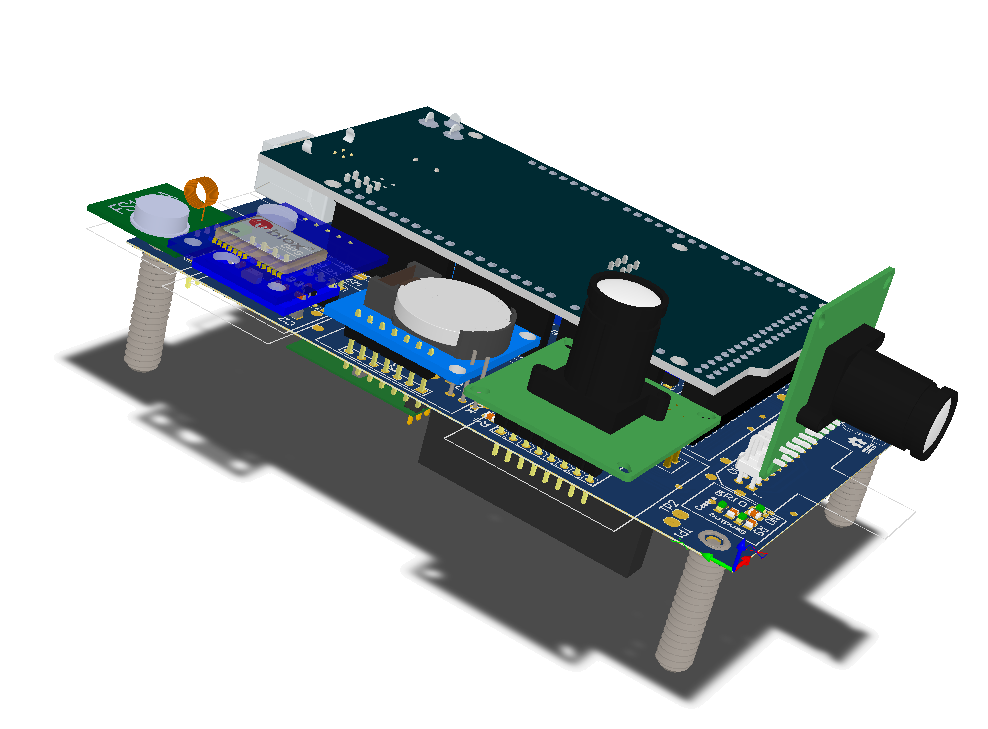
\includegraphics[scale = 0.5]{ortogonal_view}
  \caption{3D design final PCB}
  \label{fig:pcb}
\end{figure}
\begin{figure}[h]
  \centering
  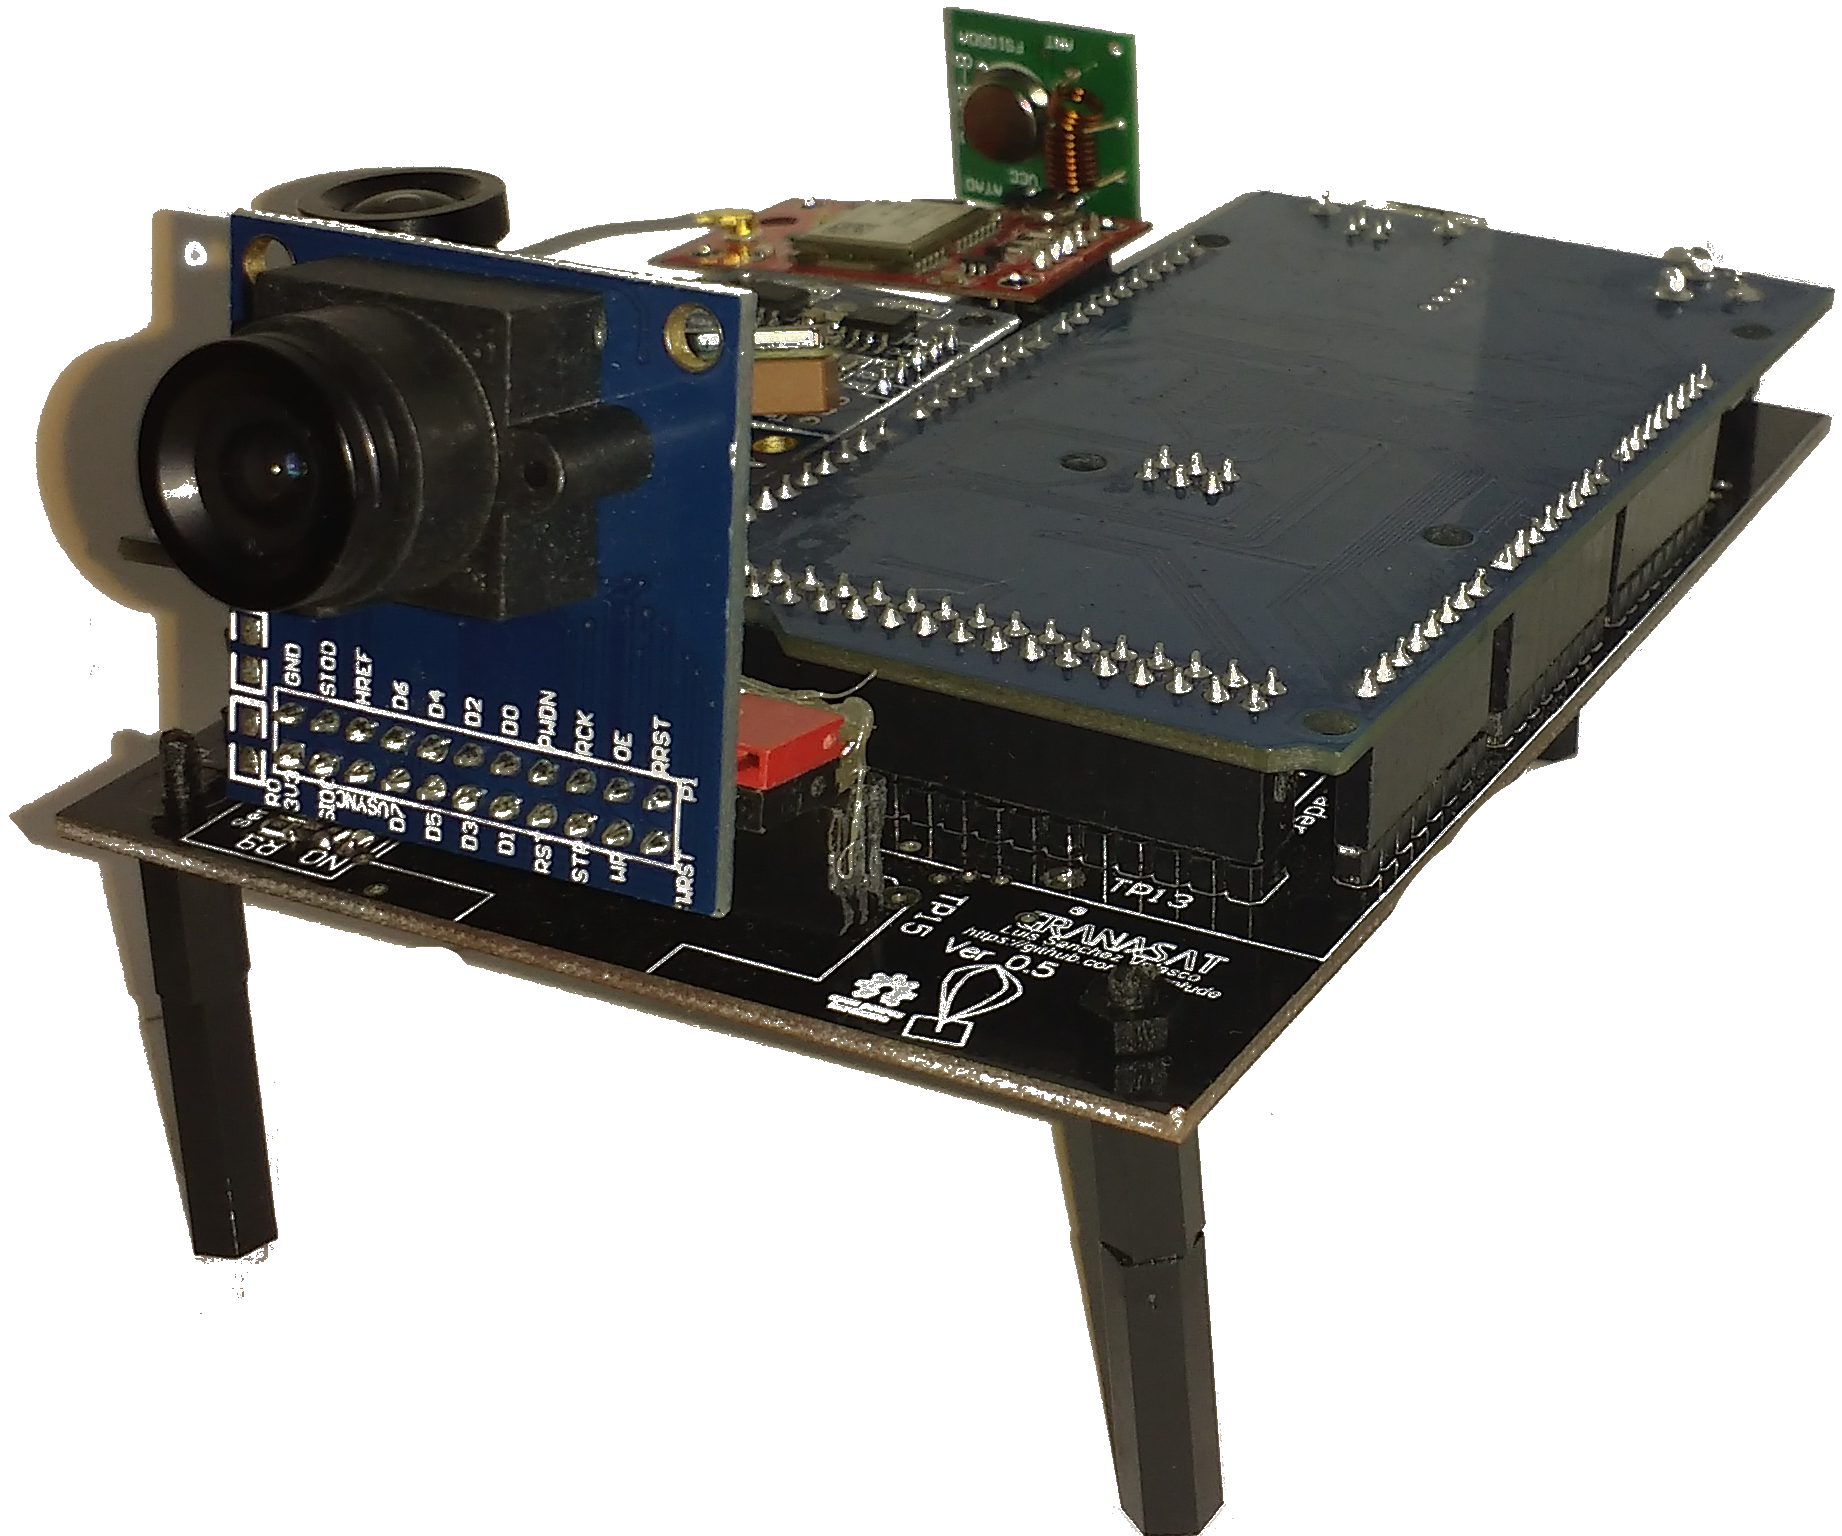
\includegraphics[scale = 0.15]{final}
  \caption{Manufactured PCB}
  \label{fig:mpcb}
\end{figure}
%\section{Other information}

%\subsection{Review}

%Alice approaches Wonderland as an anthropologist, but maintains a strong sense of noblesse oblige that comes with her class status. She has confidence in her social position, education, and the Victorian virtue of good manners. Alice has a feeling of entitlement, particularly when comparing herself to Mabel, whom she declares has a ``poky little house," and no toys. Additionally, she flaunts her limited information base with anyone who will listen and becomes increasingly obsessed with the importance of good manners as she deals with the rude creatures of Wonderland. Alice maintains a superior attitude and behaves with solicitous indulgence toward those she believes are less privileged.

%----------------------------------------------------------------------------------------

\end{document}
